%=============================================================================
% ICIIBMS 2026 -- IEEE conference format, DOUBLE BLIND.
% No author names, affiliations, or acknowledgements until camera-ready.
% Check PDF metadata before submission: the CFP forbids identifying
% information "in the embedded PDF data".
%=============================================================================
\documentclass[conference,a4paper]{IEEEtran}
\IEEEoverridecommandlockouts

\usepackage{cite}
\usepackage{amsmath,amssymb}
\usepackage{graphicx}
\usepackage{booktabs}
\usepackage{xcolor}
\usepackage[hidelinks]{hyperref}
\usepackage{fancyhdr}

% ICIIBMS conference header/footer follows the supplied IEEE Word template.
\setlength{\headheight}{12pt}
\setlength{\footskip}{76pt}
\newcommand{\IEEEfooter}{%
  \begin{tabular}[b]{c}
    \makebox[\dimexpr\textwidth-12pt\relax][l]{%
      \makebox[0.44\textwidth][c]{%
        \raisebox{6pt}{\parbox[b]{0.44\textwidth}{\centering\rule{\linewidth}{0.4pt}\\[-1pt]\footnotesize\bfseries \textcopyright 2026 IEEE}}}%
      \hspace{0.025\textwidth}%
      \raisebox{-10pt}{
\includegraphics[width=0.75in]{figures/ieee-logo.jpg}}}\\[35pt]
    \thepage
  \end{tabular}}
\fancypagestyle{iciibms}{%
  \fancyhf{}
  \fancyhead[C]{\footnotesize ICIIBMS 2026, Track 3: Bioinformatics, Bioengineering, Medical Imaging, Neuroscience \& Natural Science, Okinawa, Japan, Nov. 21--24, 2026}
  \fancyfoot[C]{\IEEEfooter}
  \renewcommand{\headrulewidth}{0pt}
  \renewcommand{\footrulewidth}{0pt}}
\setlength{\textfloatsep}{6pt plus 2pt minus 2pt}
\setlength{\dbltextfloatsep}{6pt plus 2pt minus 2pt}
\setlength{\floatsep}{4pt plus 1pt minus 1pt}
\setlength{\intextsep}{4pt plus 1pt minus 1pt}

%=============================================================================
% ANONYMITY SWITCH
%   \anontrue   -> INITIAL submission (double blind). Use this to submit.
%   \anonfalse  -> CAMERA-READY, after acceptance only.
% ICIIBMS forbids identifying information "anywhere in the manuscript, abstract,
% or in the embedded PDF data", so also drop the pdfauthor/pdftitle overrides in
% the hyperref line above when switching to camera-ready.
%=============================================================================
\newif\ifanon
\anonfalse         % camera-ready author version

\begin{document}

\title{Sign Blindness and the Limits of Overlap Metrics for Ejection Fraction in Automated Echocardiography}

\ifanon
  \author{\IEEEauthorblockN{Anonymous Submission}
  \IEEEauthorblockA{Paper ID: XXXX}}
\else
  \author{%
  \IEEEauthorblockN{Nafis Naufal Rahman}
  \IEEEauthorblockA{\textit{Faculty of Computer Science}\\
  \textit{Department of Information Engineering}\\
  University of Brawijaya\\
  Malang, Indonesia \\
  nafisnaufal1426@student.ub.ac.id\\
  ORCID: \href{https://orcid.org/0009-0007-4629-9369}{0009-0007-4629-9369}}
  \and
  \IEEEauthorblockN{Dionisius Seraf Saputra}
  \IEEEauthorblockA{\textit{Faculty of Computer Science}\\
  \textit{Department of Information Systems}\\
  University of Brawijaya\\
  Malang, Indonesia \\
  dionisiusve32@student.ub.ac.id\\
  ORCID: \href{https://orcid.org/0009-0008-2331-616X}{0009-0008-2331-616X}}
  \and
  \IEEEauthorblockN{Novanto Yudistira}
  \IEEEauthorblockA{\textit{Faculty of Computer Science}\\
  \textit{Department of Information Engineering}\\
  University of Brawijaya\\
  Malang, Indonesia \\
  yudistira@ub.ac.id\\
  ORCID: \href{https://orcid.org/0000-0001-5330-5930}{0000-0001-5330-5930}}
  }
\fi

\maketitle
\pagestyle{iciibms}
\thispagestyle{iciibms}
\small

%-----------------------------------------------------------------------------
\begin{abstract}
Automated left-ventricular segmentation is almost universally evaluated with the Dice
coefficient, yet the clinical output derived from it is ejection fraction (EF). We show
that Dice alone is insufficient as a metric for EF error and identify the mechanism: Dice
is blind to the sign of a boundary error, whereas EF, a normalised difference of two
volumes, is not. Perturbing expert contours with unbiased boundary noise alone reproduces
the observed decoupling, with R squared 0.27 simulated versus 0.19 measured, and
end-diastolic and end-systolic errors of opposite sign produce 2.0 times the EF error of
same-sign errors while being indistinguishable by Dice. Across two institutions and
10,524 patients (CAMUS and EchoNet-Dynamic), 7.5 percent of patients in the best Dice
quartile still receive a large EF error above 10 points, and across four models spanning
4 times capacity, Dice varies by 0.47 percent while the rate of such errors varies by
36.6 percent. We benchmark against human variability: our EF error (6.69 points) is
comparable to published echocardiographer-versus-CMR differences (6 to 7 points), so
models are not uniquely unreliable but the reported metric does not identify which patients
are affected. On CAMUS, expert-graded poor acoustic windows raise the rate of large EF
errors 3.3-fold (adjusted OR 4.89, 95 percent confidence interval 2.49 to 9.60, p below
0.0001; N = 500) after controlling for reference EF, while mean Dice falls by only 3.5
percent relative. We also show that CAMUS cannot power a robustness claim (207 poor-quality
patients per arm required, 47 available), and that image-quality assessment does not
transfer between echocardiography datasets. We recommend reporting clinical-endpoint
error against a human-variability reference band alongside Dice. Code and configuration
files are publicly available at: \href{https://github.com/yukienjoyer7/sign-blindness-reproducibility}{github.com/yukienjoyer7/sign-blindness-reproducibility}.
\end{abstract}

\begin{IEEEkeywords}
echocardiography, ejection fraction, image segmentation, evaluation metrics, statistical
power, clinical deployment
\end{IEEEkeywords}

%-----------------------------------------------------------------------------
\section{Introduction}

Echocardiography is the most widely used cardiac imaging modality, and left-ventricular
ejection fraction is its most consequential output. EF thresholds define the three
heart-failure categories in current guidelines, namely reduced ($<40\%$), mildly reduced
($40$ to $49\%$) and preserved ($\geq 50\%$) ejection fraction \cite{mcdonagh2021}, and
those categories in turn govern eligibility for implantable defibrillators and for
disease-modifying drug therapy. EF is also the primary surveillance measure during
cardiotoxic chemotherapy \cite{thavendiranathan2013}. A measurement error of ten EF points
is therefore not an abstract inaccuracy; it can move a patient across a treatment boundary.

Deep learning now segments the left ventricle with Dice coefficients above $0.92$ on public
benchmarks \cite{leclerc2019,ouyang2020,isensee2021}, a level routinely described as
approaching expert agreement. Reported progress in this literature is dominated by overlap
metrics, principally Dice \cite{dice1945,milletari2016} and occasionally boundary distances
\cite{taha2015}.

EF, however, is not a segmentation. It is a ratio computed from segmentations at two
cardiac phases,
\begin{equation}
\mathrm{EF} = \frac{V_{\mathrm{ED}} - V_{\mathrm{ES}}}{V_{\mathrm{ED}}} \times 100 ,
\label{eq:ef}
\end{equation}
where the volumes follow Simpson's method of discs as recommended by the American Society
of Echocardiography and the European Association of Cardiovascular Imaging
\cite{lang2015}. Because Eq.~\eqref{eq:ef} is a non-linear functional of two independent
segmentations, errors at end-diastole and end-systole combine unfavourably: a
segmentation that is excellent by overlap can still produce a clinically wrong EF if its
errors are distributed asymmetrically between phases. Figure~\ref{fig:teaser} shows two
patients from the same model whose Dice scores differ by $0.009$ and whose EF errors differ
by $22$ points.

Dice measures overlap magnitude but does not encode whether a contour is displaced inward
or outward. This distinction matters for EF because end-diastolic and end-systolic errors
enter the EF calculation with different signs. We therefore examine whether this lost
directional information explains the weak association between Dice and EF error.

This paper asks a simple question with an uncomfortable answer: \emph{how much does the
metric the field reports tell us about the quantity clinicians act on?}

\medskip\noindent\textbf{Contributions.}
\begin{enumerate}
\item We identify the \emph{mechanism} behind the Dice-to-EF decoupling: Dice is blind to
      the sign of a boundary error while EF is not. A null model using only unbiased
      boundary noise on expert contours is consistent with the observed decoupling, and a
      sign-aware phase-error companion recovers part of the EF-error association
      (Section~\ref{sec:mechanism}).
\item We separate two claims that are easily conflated. \emph{Within} a model across
      patients, Dice poorly predicts EF error; \emph{across} models, Dice varies by
      $0.47\%$ while the rate of large EF errors varies by $36.6\%$
      (Sections~\ref{sec:decoupling} and \ref{sec:mechanism}).
\item We benchmark against human variability rather than in isolation, and find the model's
      EF error comparable to published echocardiographer-versus-CMR differences. The
      problem is not that models are uniquely unreliable but that Dice cannot indicate
      which patients are affected (Section~\ref{sec:clinical}).
\item We show expert-graded poor acoustic windows raise the rate of large EF errors
      3.3-fold, and that this survives adjustment for disease severity (adjusted
      OR $4.89$, 95\% CI $[2.49,9.60]$, $N=500$) (Section~\ref{sec:quality}).
\item We report a power analysis showing CAMUS cannot support method claims about
      poor-quality robustness, with a worked false negative
      (Section~\ref{sec:power}), and that image-quality assessment does not transfer
      between datasets (Section~\ref{sec:transfer}).
\end{enumerate}

%-----------------------------------------------------------------------------
\begin{figure}[t]
\centering
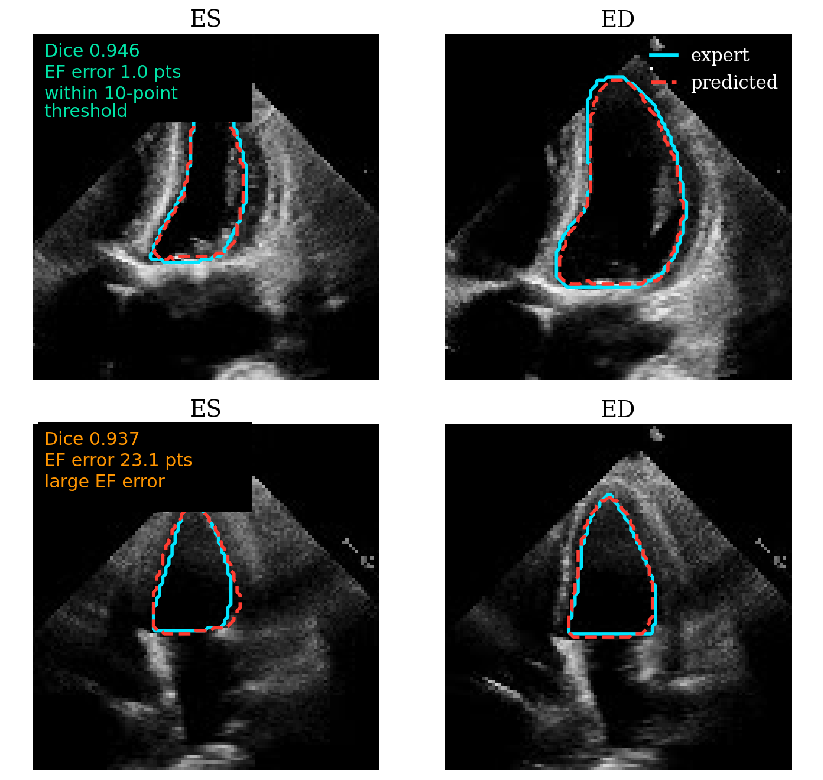
\includegraphics[width=\columnwidth]{figures/fig1_teaser.pdf}
\caption{Two EchoNet-Dynamic patients segmented by the same model. Expert contours in cyan,
predictions in dashed red. \textbf{Top:} Dice $0.946$, EF error $1.0$ points.
\textbf{Bottom:} Dice $0.937$, EF error $23.1$ points. A Dice difference of $0.009$, which
any conventional evaluation would treat as noise, separates a measurement within the
10-point threshold from one with a large EF error. The latter can also cause
EF-category misclassification. These are
\emph{selected} cases: the lower panel is the largest EF error within a narrow Dice band,
chosen to illustrate the mechanism, not a typical outcome.}
\label{fig:teaser}
\end{figure}

%-----------------------------------------------------------------------------
\section{Related Work}

\textbf{Echocardiographic segmentation and EF estimation.}
CAMUS \cite{leclerc2019} established the standard 2D benchmark with 500 patients, two
apical views and expert quality grades. EchoNet-Dynamic \cite{ouyang2020} provides
10{,}030 apical four-chamber videos with expert end-diastolic and end-systolic tracings and
demonstrated beat-to-beat EF assessment from video. Subsequent work has explored
transformer architectures for EF regression \cite{reynaud2021}, broader phenotype
prediction from echocardiograms \cite{ghorbani2020}, and fully automated interpretation
pipelines evaluated in clinical practice \cite{zhang2018,asch2019}. Architectural progress
continues to be measured predominantly by Dice, with self-configuring pipelines such as
nnU-Net \cite{isensee2021} setting the standard for segmentation quality across
biomedical tasks and U-Net \cite{ronneberger2015} remaining the dominant backbone.

\textbf{Metric criticism in medical imaging.}
A growing literature argues that overlap metrics are poorly aligned with clinical utility.
Taha and Hanbury \cite{taha2015} catalogued the properties of segmentation metrics and
their failure modes, and the recent Metrics Reloaded effort
\cite{maierhein2024,reinke2024} provides problem-driven recommendations for metric
selection, emphasising boundary sensitivity, small-structure bias and class imbalance.
Painchaud et al.\ \cite{painchaud2020} showed that deep segmentation models routinely
produce anatomically impossible cardiac shapes that overlap metrics do not penalise. Our
contribution is complementary and empirical: rather than arguing from metric properties, we
measure how much the reported metric predicts a specific downstream clinical quantity, at
scale, across two institutions.

\textbf{Image quality in echocardiography.}
Poor acoustic windows are common in obese, chronic obstructive pulmonary disease and
intensive-care patients, and quality is the dominant practical constraint on
echocardiographic measurement \cite{lang2015}. Automated quality assessment has been
studied as an acquisition guidance tool \cite{abdi2017}, with the best regional estimator
reaching Spearman $\rho = 0.69$ against expert grades where inter-observer agreement is
$\rho = 0.63$ \cite{rogers2024}. Whether such models transfer across datasets has not, to
our knowledge, been reported.

\textbf{Observer variability as a reference scale.}
Any claim about measurement error requires a yardstick. Sequential echocardiographic EF
assessment has substantial temporal variability even between human readers, with reported
test-retest confidence intervals for 2D biplane EF wide enough to obscure clinically
meaningful change \cite{thavendiranathan2013}. We therefore report Bland--Altman limits of
agreement \cite{blandaltman1986}, the standard instrument for method comparison in clinical
measurement, rather than mean error alone.

%-----------------------------------------------------------------------------
\section{Materials and Methods}

\subsection{Datasets}
\textbf{CAMUS} \cite{leclerc2019} contains 500 patients imaged at a single European centre,
with apical two-chamber and four-chamber views at end-diastole and end-systole. Expert
contours cover the LV endocardium, myocardium and left atrium. Critically for this study,
each view carries an expert cardiologist quality grade: across 1000 patient-view records,
$50.5\%$ are Good, $37.9\%$ Medium and $11.6\%$ Poor. Reference EF is provided per patient.

\textbf{EchoNet-Dynamic} \cite{ouyang2020} contains 10{,}030 apical four-chamber videos
acquired during routine care at a single US centre, with expert tracings at two phases in
the clinical 21-line format and reference EF, end-systolic and end-diastolic volumes. We
use the official $7465 / 1288 / 1277$ split. Videos are distributed pre-resized to
$112 \times 112$.

Together the two datasets span two continents, different vendors, different annotation
protocols and both mono- and biplane EF conventions, which is what allows the central
finding to be tested for institutional robustness rather than assumed.

\subsection{Ejection fraction measurement}
Let $F(M_{\mathrm{ED}},M_{\mathrm{ES}})$ denote the same Simpson measurement procedure
applied to the end-diastolic and end-systolic masks \cite{lang2015}. For expert and
predicted masks, respectively, we define
\begin{equation}
\mathrm{EF}_{\mathrm{ref}} = F(M^{\mathrm{ref}}_{\mathrm{ED}},M^{\mathrm{ref}}_{\mathrm{ES}}),
\quad
\mathrm{EF}_{\mathrm{pred}} = F(M^{\mathrm{pred}}_{\mathrm{ED}},M^{\mathrm{pred}}_{\mathrm{ES}}),
\end{equation}
and the segmentation-induced endpoint is
\begin{equation}
E_{\mathrm{EF}} = \left|\mathrm{EF}_{\mathrm{pred}}-\mathrm{EF}_{\mathrm{ref}}\right|.
\end{equation}
Thus, EF error is derived from the two mask measurements and is not a separately
annotated label. The dataset-provided EF is used only to validate the reconstruction
procedure. For
CAMUS we use the biplane formulation. The long axis is located anatomically, from the
mitral-annulus midpoint (identified as the LV to left-atrium interface) to the apex, and
disc diameters are measured perpendicular to that axis. Assuming instead that the long axis
is vertical, as an axis-aligned implementation would, costs several EF points because
apical views are routinely tilted. For EchoNet we use the monoplane formulation matching
the dataset's own 21-line tracing protocol.

Validating the measurement pipeline on \emph{expert} contours is essential, because a
mismeasuring pipeline would silently attribute its own error to the model. On EchoNet our
reconstruction reproduces the dataset's reference EF at $r = 0.971$ with mean absolute
error $1.05$ EF points, so measured error is dominated by segmentation rather than by the
EF computation. On CAMUS the biplane pipeline attains $r = 0.977$ with a constant additive
offset of $+8.3$ points, arising from a systematic difference in the ESV to EDV ratio.
Because the offset is additive (slope $0.9975$, residual standard deviation $2.61$),
\textbf{all reported EF errors are computed by applying the identical pipeline to predicted
and to expert masks}, so the $+8.3$-point offset cancels exactly. The paired comparison
therefore isolates the EF difference associated with the segmentation masks under our
measurement procedure, rather than absolute agreement with the dataset-provided EF.

We use a threshold of $10$ EF points, approximately the width of a heart-failure category
boundary \cite{mcdonagh2021}, to define a \textbf{large EF error ($>10$ points)}. We
separately use \textbf{EF-category misclassification} for a patient crossing one of the
guideline thresholds. A large EF error is a measurement endpoint, not a direct clinical
outcome, and is interpreted against the variability of the measurement it replaces. We
also report the large-EF-error rate for every threshold from 0 to 20 points, with 10 points
marked as the reference threshold.

\subsection{Human variability reference band}
Automated EF error must be judged against how much human readers disagree, not against
zero. Reported 2D echocardiographic EF variability is substantial: inter-observer
variability of up to roughly $14$ EF points, absolute echocardiography-versus-CMR
differences of $7$ points falling to $6$ after a dedicated training programme, and
categorical EF misclassification against CMR of $56\%$ falling to $47\%$ after that same
training \cite{thavendiranathan2013b}. Sequential 2D assessment carries temporal
variability above $10$ EF points \cite{thavendiranathan2013}. We report these as a
reference band throughout. They are not directly comparable to our numbers, since they use
CMR as reference where we use expert echocardiographic contours, but they establish the
scale on which automated error should be read.

\subsection{Analysis plan}
The primary analysis was pre-specified: the association between Dice and EF error, and the
association between expert quality grade and the rate of large EF errors. The null model,
the model sweep and the severity-adjusted analysis were added in response to review and are
reported as such. Reported $p$-values are not corrected for multiplicity; the headline
associations have $p < 10^{-4}$ and would survive any standard correction, but exploratory
comparisons should be read as descriptive.

\subsection{Segmentation models}
We train a 2D U-Net \cite{ronneberger2015} with 7.76M parameters, group normalisation and a
combined Dice and cross-entropy objective \cite{milletari2016}, separately on each dataset.

On CAMUS we use 5-fold \emph{patient-level} cross-validation so that all 500 patients are
evaluated out of fold. Frame-level splitting would leak badly here, because a patient's
four frames share one acoustic window and therefore share their quality grade almost by
construction. On EchoNet we use the official split.

Test performance is Dice $0.899$ on CAMUS across three structures and $0.924$ on EchoNet for
the LV, both consistent with published results for these benchmarks
\cite{leclerc2019,ouyang2020}. The models are therefore representative of the literature
rather than weak baselines, which matters because a deliberately poor model would
exaggerate any decoupling.

\subsection{Image quality model}
To test whether quality labels can be transported between datasets, we train an ordinal
quality grader on CAMUS expert grades. The network is a small convolutional encoder with a
cumulative-logit head, which respects the ordering of the grades so that confusing Good
with Poor is penalised more heavily than confusing Good with Medium. The grader observes
only the image, never EF or segmentation, so a predicted grade cannot smuggle in outcome
information and manufacture the correlation under test. Splits are again by patient.

\subsection{Statistics}
Proportions are compared with Fisher's exact test, distributions with the Mann--Whitney $U$
test, and all point estimates carry percentile bootstrap $95\%$ confidence intervals from
$10^4$ resamples. Method agreement is reported as Bland--Altman bias and limits of
agreement \cite{blandaltman1986}. Power calculations use the normal approximation for two
proportions at $\alpha = 0.05$.

%-----------------------------------------------------------------------------
\section{Within-Model Decoupling of Dice and EF Error}
\label{sec:decoupling}

\begin{figure*}[t]
\centering
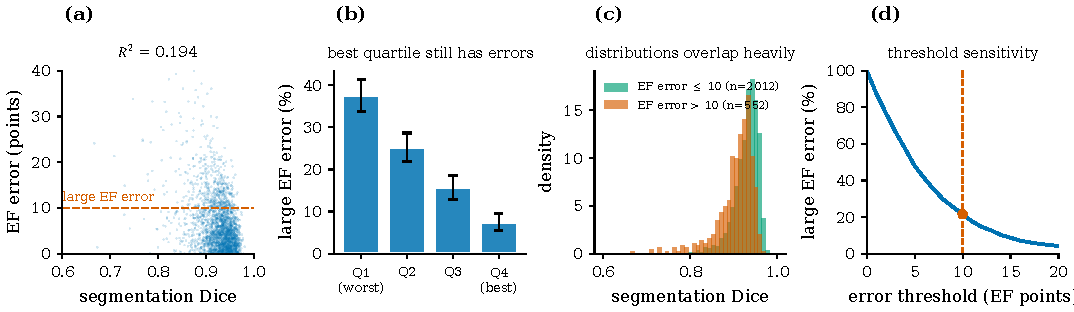
\includegraphics[width=\textwidth]{figures/fig2_decoupling.pdf}
\caption{Decoupling of overlap and EF error on 2{,}564 held-out EchoNet-Dynamic
patients. \textbf{(a)} EF error against Dice, showing a weak relationship
($R^2 = 0.194$). \textbf{(b)} Rate of large EF error by Dice quartile: even the
best quartile has a $7.5\%$ rate. \textbf{(c)} Dice distributions for cases above and
below the threshold overlap almost completely. \textbf{(d)} The large-EF-error rate
decreases continuously as the threshold increases; the dashed line marks 10 points.}
\label{fig:decoupling}
\end{figure*}

On 2{,}564 held-out EchoNet patients the model attains Dice $0.924$, matching published
performance \cite{ouyang2020}. Yet EF mean absolute error is $6.69$ points
($95\%$ CI $[6.44, 6.98]$) and \textbf{$21.5\%$ of patients have a large EF error}
above 10 points.

Dice and EF error are only weakly related, with Spearman $\rho = -0.308$
($p = 2.1 \times 10^{-57}$) and $R^2 = 0.194$. The relationship is statistically
unambiguous but practically weak: more than $80\%$ of the variance in the clinical endpoint
is invisible to the reported metric.

Figure~\ref{fig:decoupling}(b) makes the consequence concrete. Stratifying by Dice
quartile, the rate of large EF error falls only from $37.5\%$ to $7.5\%$ across the
entire range of segmentation quality. Patients with a large EF error have mean Dice
$0.9046$ against $0.9293$ for the rest, so \textbf{a difference of $0.025$ Dice separates
cases below and above the threshold}, well inside the range most papers report as noise.
Figure~\ref{fig:decoupling}(c) shows the two distributions overlapping almost entirely,
which is the same fact stated as a classification problem: Dice is a poor discriminator of
large EF error.

\subsection{Replication across institutions}
The same pattern holds on CAMUS, with biplane rather than monoplane EF, a different vendor,
a different population and a different annotation protocol. Overall $14.4\%$ of CAMUS
patients have a large EF error while mean Dice is $0.899$. That two independent
datasets agree suggests the decoupling is a property of the EF computation in
Eq.~\eqref{eq:ef} rather than of a particular cohort or model.

%-----------------------------------------------------------------------------
\section{The Mechanism: Dice Is Sign-Blind}
\label{sec:mechanism}

\begin{figure*}[t]
\centering
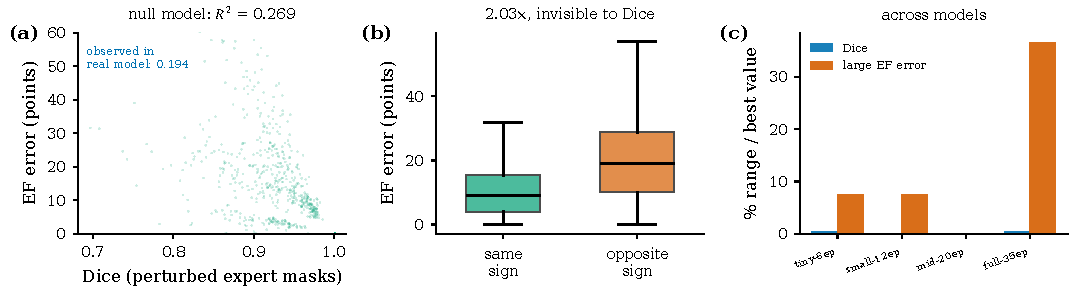
\includegraphics[width=\textwidth]{figures/fig5_mechanism.pdf}
\caption{Why the decoupling occurs. \textbf{(a)} A null model that perturbs \emph{expert}
contours with unbiased signed boundary noise, involving no trained model at all, reproduces
the observed decoupling ($R^2 = 0.269$ versus $0.194$ measured). \textbf{(b)} End-diastolic and
end-systolic boundary errors of opposite sign produce $2.03\times$ the EF error of same-sign
errors; Dice scores the two cases identically. \textbf{(c)} Across four models spanning
$4\times$ capacity and $6\times$ training length, Dice varies by $0.47\%$ while the rate of
large EF errors varies by $36.6\%$. The spread is the range divided by the best value:
maximum for Dice and minimum for error rates.}
\label{fig:mechanism}
\end{figure*}

Sections~\ref{sec:decoupling} established \emph{that} Dice and EF error are weakly related.
This section establishes \emph{why}, which turns a descriptive observation into a
prediction that generalises beyond our data.

\subsection{Sign-blindness}
Dice is a set-overlap measure and is therefore insensitive to the direction of a boundary
error: a contour uniformly too large and one uniformly too small by the same amount receive
the same score. Ejection fraction is not sign-insensitive. In Eq.~\eqref{eq:ef}, an
over-segmented end-diastolic frame inflates $V_{\mathrm{ED}}$ and pushes EF up, whereas an
over-segmented end-systolic frame inflates $V_{\mathrm{ES}}$ and pushes EF down. Errors of
the same sign at both phases partly cancel in the ratio; errors of opposite sign compound.
Dice cannot distinguish these two situations even in principle.

The same point follows from a first-order expansion. Write the predicted volumes as
$\widehat{V}_{\mathrm{ED}}=V_{\mathrm{ED}}(1+\epsilon_{\mathrm{ED}})$ and
$\widehat{V}_{\mathrm{ES}}=V_{\mathrm{ES}}(1+\epsilon_{\mathrm{ES}})$, where the two
$\epsilon$ values are signed relative errors. With $q=V_{\mathrm{ES}}/V_{\mathrm{ED}}$,
\begin{equation}
\widehat{\mathrm{EF}}
\approx \mathrm{EF}+100q(\epsilon_{\mathrm{ED}}-\epsilon_{\mathrm{ES}}).
\label{eq:first_order}
\end{equation}
Thus matching signs can partially cancel through the difference, whereas opposite signs
accumulate. Dice records overlap magnitude but not this direction.

\subsection{A null model}
To test whether this alone explains the observed decoupling, we discard the trained model
entirely. We take \emph{expert} contours, perturb each frame independently by a signed
morphological dilation or erosion drawn from a zero-mean Gaussian with $\sigma=1.6$ pixels,
and recompute both Dice and EF. There is no learning, no image content and no systematic
volume bias.

The result reproduces the measured relationship: $R^2 = 0.269$ between Dice and EF error
under pure boundary noise, against $R^2 = 0.194$ measured with the real model
(Figure~\ref{fig:mechanism}(a)). This is consistent with unbiased boundary noise and does
not establish mathematical necessity.

The mechanism is directly visible in the same simulation
(Figure~\ref{fig:mechanism}(b)). Cases whose end-diastolic and end-systolic perturbations
share a sign incur a mean EF error of $11.7$ points; cases with opposite signs incur
$23.7$ points, a factor of $2.03$. Dice is identical in distribution across the two groups
by construction.

We also ran a sensitivity sweep at $\sigma=0.5$, $1.0$, $1.6$, $2.0$ and $3.0$ pixels.
Across the independent-noise runs, $R^2$ ranged from $0.240$ to $0.359$ and the
same-sign fraction ranged from $0.497$ to $0.526$. Using the empirical signed ED/ES
correlation $\rho=0.554$ in a correlated-noise variant, $R^2$ ranged from $0.082$ to
$0.100$ and the same-sign fraction from $0.684$ to $0.704$; each run contained 2,564
patients. These sensitivity results show that the direction of the effect is not tied to
one noise magnitude, while the correlated variant makes clear that the ED/ES dependence
changes the expected association.

As a sign-aware companion, we computed signed relative phase errors and formed
$S=\epsilon_{\mathrm{ED}}-\epsilon_{\mathrm{ES}}$. On the 2,564 held-out patients, the
empirical signed ED/ES correlation was $0.554$, and $S$ correlated with EF error at
Pearson $r=-0.443$ ($R^2=0.196$); $70.9\%$ of patients had same-sign phase errors. This
companion is not a replacement for Dice, but it exposes the directional information that
Dice omits.

\subsection{Within-model and across-model claims}
The claim ``Dice does not predict clinical error'' admits two readings, which we separate
because only one was supported by our original analysis.

\emph{Within} a model, across patients: a patient's Dice poorly predicts that patient's EF
error. This is what Section~\ref{sec:decoupling} measures.

\emph{Across} models: we descriptively compare four models spanning $4\times$ capacity
(widths 8 to 32) and $6\times$ training length (6 to 35 epochs). Because width and training
length change together, this sweep does not isolate the source of any performance difference.

\begin{table}[t]
\caption{Descriptive across-model comparison on the EchoNet test split. Dice is nearly
constant while the rate of large EF errors varies by more than a third. Relative spread is
the range divided by the best value: maximum for Dice and minimum for error measures.}
\label{tab:sweep}
\centering
\begin{tabular}{lccc}
\toprule
Model & Dice & EF MAE & Large EF error $>10$ \\
\midrule
tiny (w8, 6 ep)    & 0.9189 & 6.85 & 21.4\% \\
small (w12, 12 ep) & 0.9230 & 6.69 & 21.4\% \\
mid (w20, 20 ep)   & 0.9232 & 6.75 & \textbf{19.9\%} \\
large (w32, 35 ep) & 0.9195 & \textbf{8.00} & \textbf{27.2\%} \\
\midrule
relative spread    & \textbf{0.47\%} & 19.6\% & \textbf{36.6\%} \\
\bottomrule
\end{tabular}
\end{table}

Table~\ref{tab:sweep} shows a $0.47\%$ relative spread in Dice against a $36.6\%$ relative
spread in the rate of large EF errors. The largest and longest-trained model has the
highest observed error rate despite mid-range Dice, but the confounded sweep does not identify
the cause. With only four models a correlation test is underpowered
($p = 0.43$) and we draw no conclusion about the direction of any across-model
relationship. The descriptive observation stands on its own: \textbf{models that are
indistinguishable by Dice differ by a third in large-EF-error rate.}

\section{Clinical Consequences}
\label{sec:clinical}

\begin{figure*}[t]
\centering
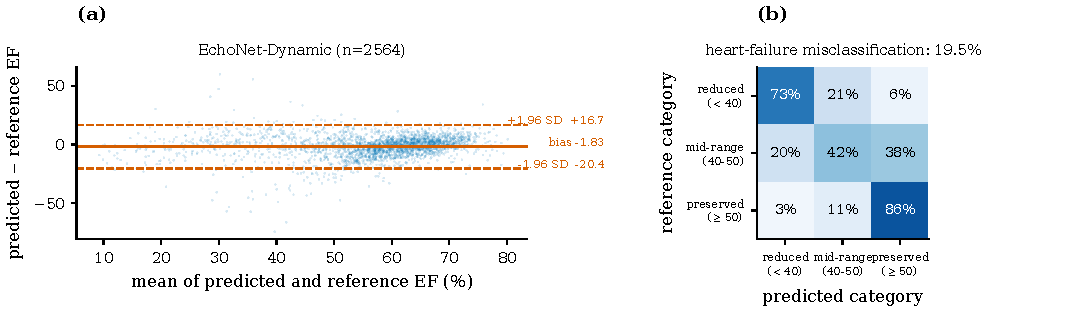
\includegraphics[width=\textwidth]{figures/fig4_bland_altman.pdf}
\caption{Clinical translation on EchoNet-Dynamic. \textbf{(a)} Bland--Altman analysis: bias
is small ($-1.83$ EF points) but the limits of agreement span $37$ points.
\textbf{(b)} Heart-failure category assignment against the reference; $19.5\%$ of patients
are placed in the wrong category.}
\label{fig:ba}
\end{figure*}

Mean error understates the clinical problem, because a method can be unbiased on average
and still have a large individual-patient error. Bland--Altman analysis
(Figure~\ref{fig:ba}(a)) shows a small bias of $-1.83$ EF points but limits of agreement of
$[-20.4, +16.7]$, a span of $37$ EF points. For context, that interval is wider than the
entire mildly-reduced heart-failure category.

\subsection{Against the human reference band}
These numbers must be read against how much humans disagree. Published
echocardiography-versus-CMR absolute EF differences are $6$ to $7$ points
\cite{thavendiranathan2013b} and our model's $6.69$ point MAE falls within that range;
reported human inter-observer variability reaches roughly $14$ points. The reference
standards differ, ours being expert echocardiographic contours rather than CMR, so these
are not interchangeable figures. But the comparison forbids one conclusion that the raw
numbers might otherwise invite: \textbf{these models are not uniquely unreliable, and
describing every error above 10 points as a direct clinical consequence would misrepresent them.}
Human EF-category misclassification
against CMR has been reported at $47\%$ to $56\%$ \cite{thavendiranathan2013b}, higher than
the $19.5\%$ we measure against expert contours.

The problem this paper identifies is therefore not that automated EF is unusually bad. It
is that \emph{the reported metric does not tell you which patients are affected}, and unlike a
human reader, an automated pipeline offers no accompanying signal of low confidence.

The decisive translation is categorical. Assigning each patient to reduced, mildly reduced
or preserved EF using guideline thresholds \cite{mcdonagh2021},
\textbf{$19.5\%$ of patients are placed in the wrong category}
(Figure~\ref{fig:ba}(b)). Since category membership governs defibrillator eligibility and
drug therapy, this is the number a clinician would want to see reported, and it is not
recoverable from a Dice score of $0.924$.

\subsection{Mildly reduced EF is where the model is weakest}
The errors are unevenly distributed across categories in a clinically unfavourable
way. Preserved EF is assigned correctly in $86\%$ of cases and reduced EF in $73\%$, but the
mildly-reduced category is recovered in only $42\%$ of cases, with $38\%$ of those patients
promoted to preserved and $20\%$ demoted to reduced. The mildly-reduced band is both the
narrowest of the three and the one in which treatment decisions are least settled, so the
model is least reliable precisely where the clinical question is hardest.

%-----------------------------------------------------------------------------
\section{Image Quality Shifts Large EF Error, Not Dice}
\label{sec:quality}

\begin{figure*}[t]
\centering
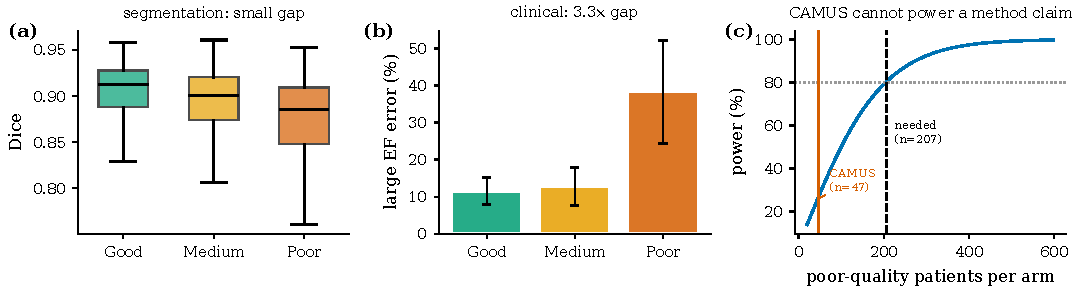
\includegraphics[width=\textwidth]{figures/fig3_quality_power.pdf}
\caption{CAMUS, stratified by expert cardiologist quality grade. \textbf{(a)} Dice degrades
only slightly. \textbf{(b)} The rate of large EF error rises 3.3-fold.
\textbf{(c)} Power to detect a realistic improvement on the poor-quality stratum: CAMUS
contains 47 such patients where about 207 per arm are required.}
\label{fig:quality}
\end{figure*}

CAMUS uniquely provides expert quality grades, which allows the decoupling to be examined
against a clinically meaningful covariate. Out of fold across all 500 patients,
segmentation degrades modestly with quality: Dice $0.899$, $0.890$ and $0.870$ for Good,
Medium and Poor respectively.

The clinical picture is entirely different (Table~\ref{tab:quality}). The rate of large EF
error rises from $11.9\%$ to $38.3\%$, an odds ratio of $4.59$
($p = 1.6 \times 10^{-5}$). A $3.5\%$ relative degradation in the reported metric
accompanies a $233\%$ relative increase in the large-EF-error rate.

\begin{table}[t]
\caption{CAMUS: segmentation versus clinical degradation by expert quality grade.}
\label{tab:quality}
\centering
\begin{tabular}{lccc}
\toprule
Quality & Dice & EF MAE ($95\%$ CI) & Large EF error \\
\midrule
Good    & 0.899 & 5.02 $[4.49, 5.60]$ & 11.5\% \\
Medium  & 0.890 & 5.23 $[4.49, 6.01]$ & 12.7\% \\
Poor    & 0.870 & 7.35 $[5.76, 8.96]$ & \textbf{38.3\%} \\
\midrule
\multicolumn{4}{l}{Good and Medium vs.\ Poor: OR $4.59$, Fisher $p = 1.6 \times 10^{-5}$}\\
\bottomrule
\end{tabular}
\end{table}

Poor acoustic windows are not distributed at random across patients. Mean EF is $39.5$ in
the Poor stratum against $46.0$ in Good, reflecting that sicker patients are harder to
image, so image quality and disease severity are potentially confounded. We therefore fit a
logistic model for the probability of a large EF error with both poor-quality status and
reference EF as covariates. The quality effect survives and slightly strengthens:
\textbf{adjusted OR $4.89$} ($95\%$ CI $[2.49,9.60]$, $p = 4.0 \times 10^{-6}$) against
an unadjusted OR of $4.59$. The model used $N=500$ patients, with large EF error as the
outcome and poor quality plus reference EF as predictors; the reference-EF coefficient was
not significant ($p = 0.43$). Image quality, not disease severity, drives the association.

%-----------------------------------------------------------------------------
\section{A Power Trap in the Standard Benchmark}
\label{sec:power}

Having established that poor-quality scans fail clinically, the natural next step is a
method that improves them. We attempted exactly this, comparing physics-grounded acoustic
degradation augmentation against strong generic photometric augmentation at matched
perturbation magnitude. The acoustic simulator models shadowing, signal dropout, depth
attenuation, speckle and near-field clutter in the polar geometry of the beam, since a rib
shadow is an angular wedge originating at the transducer rather than an axis-aligned
rectangle.

The result was inconclusive, and instructively so. The rate of large EF error on
the poor stratum fell from $38.3\%$ to $29.8\%$ with generic augmentation and to $25.5\%$
with acoustic augmentation, but no comparison approached significance, with acoustic versus
generic at Fisher $p = 0.818$.

The reason is structural rather than methodological. Detecting a change from $38\%$ to
$26\%$ at $80\%$ power requires approximately \textbf{207 poor-quality patients per arm}.
CAMUS contains \textbf{47} in total with complete two- and four-chamber coverage
(Figure~\ref{fig:quality}(c)). No number of additional seeds, epochs or architectures can
recover this, because the benchmark itself cannot support the claim.

We encountered the same trap in a milder form. Evaluated on the official CAMUS split alone,
which contains only $8$ poor-quality patients with complete coverage, the quality to EF
relationship read $1.08\times$ at $p = 0.50$ and appeared absent. Cross-validation raised
the stratum to $47$ and the same effect became $1.44\times$ at $p = 0.012$. \textbf{An
underpowered null is not evidence of absence}, and published claims of robustness on small
strata of public benchmarks should be read with this in mind.

%-----------------------------------------------------------------------------
\section{Quality Assessment Does Not Transfer}
\label{sec:transfer}

To obtain the statistical power CAMUS lacks, we trained the ordinal quality grader on CAMUS
expert grades and applied it to EchoNet's 10{,}024 patients. Within CAMUS the grader reaches
Spearman $\rho = 0.664$ out of fold, between the published regional estimator at
$\rho = 0.69$ and inter-observer agreement at $\rho = 0.63$ \cite{rogers2024}. It is
therefore about as consistent with the cardiologists as they are with each other.

On EchoNet it fails on both available checks. Predicted scores collapse to mean $0.134$ with
standard deviation $0.092$, and the $90$th percentile still scores better than the CAMUS
\emph{Good} mean of $0.322$, which is not credible for 10{,}024 consecutive clinical
studies. More tellingly, the relationship inverts: the quality score correlates with EF at
$\rho = +0.063$ where CAMUS gives a clear negative association. A sign inversion is not a
calibration offset.

We attribute this primarily to resolution. CAMUS frames derive from approximately
$0.3$\,mm pixels whereas EchoNet ships videos pre-resized to $112 \times 112$, removing the
fine speckle character and endocardial border definition that quality assessment depends
on \cite{abdi2017,rogers2024}. We did not attempt histogram matching, feature alignment or
fine-tuning on pseudo-labels, so we report the failure of the direct approach rather than a
proof that transfer is impossible.

%-----------------------------------------------------------------------------
\section{Discussion}

Our results have a single practical consequence. \textbf{Segmentation papers whose stated
motivation is cardiac function should report clinical-endpoint error and large-error rates
alongside Dice.} A model at Dice $0.924$ on EchoNet, which would be presented as
state-of-the-art, has a large EF error in more than one patient in five and misclassifies
the heart-failure category of nearly one in five, while the reported metric gives almost
no warning of which patients are affected.

This is not an argument that Dice is useless. It is an argument that Dice is insufficient
as a sole endpoint whenever the clinical quantity is a non-linear functional of the
segmentation, as in Eq.~\eqref{eq:ef}. The concern is closely related to, but distinct
from, the metric-selection guidance of Metrics Reloaded \cite{maierhein2024,reinke2024}:
those works ask which overlap or boundary metric best reflects segmentation quality,
whereas we observe that even a well-chosen segmentation metric may be insufficient as a sole
indicator of the downstream clinical measurement.

\subsection{Recommendations}
\begin{enumerate}
\item Report EF mean absolute error, Bland--Altman limits of agreement
      \cite{blandaltman1986}, and the rate of errors beyond a clinically defined threshold,
      alongside Dice. These cost nothing to compute once segmentations exist.
\item Report categorical agreement against guideline thresholds \cite{mcdonagh2021} when
      the clinical use is diagnostic classification.
\item Validate the measurement pipeline itself on expert contours before attributing error
      to a model, and state the residual pipeline error.
\item Accompany any robustness claim on a small stratum with a power analysis, and treat a
      non-significant result on a small stratum as uninformative rather than negative.
\end{enumerate}

\subsection{Scope of the critique}
Our analysis targets EF derived from segmentation. EchoNet-Dynamic's own headline method
regresses EF directly from video without producing a segmentation \cite{ouyang2020}, and
such models are not subject to the sign-blindness argument in the same form, since they are
not evaluated by Dice at all. The critique applies to the large literature that reports
segmentation Dice while motivating the work by cardiac function, which includes most
CAMUS-based work, rather than to end-to-end regression approaches.

\subsection{Limitations}
Both datasets are retrospective and each comes from a single centre. The $10$-point
threshold is a convention motivated by heart-failure category width, and we report full
error distributions so other thresholds can be read off. EchoNet is single-view and
pre-downsampled, which limits both the quality analysis and achievable spatial precision.

Three limitations deserve particular emphasis. First, our reference standard is expert
echocardiographic contours rather than an independent modality, so the reference itself
carries observer variability \cite{thavendiranathan2013,thavendiranathan2013b}, and part of
what we score as model error is human disagreement. Second, we cannot separate segmentation
error from \textbf{end-diastolic and end-systolic frame selection error}. Both datasets
supply the traced frames, but any deployed system must choose them, and a phase-selection
mistake propagates directly into EF through Eq.~\eqref{eq:ef} while leaving per-frame Dice
untouched. Frame selection is therefore a competing and unmeasured contributor to the
decoupling, and plausibly an additional instance of the same principle. Third, our
across-model comparison uses four models spanning a narrow Dice range, which supports the
descriptive claim in Table~\ref{tab:sweep} but not a directional one.

Finally, our augmentation comparison is underpowered by construction and should not be read
as evidence that acoustic augmentation fails.

\section{Conclusion}

The Dice coefficient does not fully capture ejection fraction error: Dice is blind to the
sign of a boundary error while EF, a
normalised difference of two volumes, is not. A null model driven only by unbiased boundary
noise is consistent with the effect, and errors of opposite sign at the two cardiac phases produce
twice the EF error of same-sign errors while scoring identically. Across four models, Dice
varies by half a percent while the rate of large EF errors varies by more than a third.

Measured against human variability, these models are not unusually unreliable. That is
precisely the point: large errors are ordinary in magnitude but invisible to the metric the
field reports, and concentrated in identifiable patients, those with poor acoustic windows
and those near the mildly-reduced EF boundary. We recommend reporting clinical-endpoint
error against a human-variability reference band alongside Dice, and an explicit power
analysis for any robustness claim on a small stratum.

\section*{Acknowledgment}
We sincerely thank the AI Center, Universitas Brawijaya, for providing us with the
computational resources needed to conduct this research
(\href{https://aicenter.ub.ac.id/}{AI Center UB website}).

%-----------------------------------------------------------------------------
\begin{thebibliography}{00}

\bibitem{mcdonagh2021} T.~A. McDonagh \emph{et al.}, ``2021 ESC guidelines for the diagnosis
and treatment of acute and chronic heart failure,'' \emph{Eur. Heart J.}, vol.~42, no.~36,
pp.~3599--3726, 2021.

\bibitem{thavendiranathan2013} P.~Thavendiranathan, A.~D. Grant, T.~Negishi, J.~C. Plana,
Z.~B. Popovi\'{c}, and T.~H. Marwick, ``Reproducibility of echocardiographic techniques for
sequential assessment of left ventricular ejection fraction and volumes,'' \emph{J. Am.
Coll. Cardiol.}, vol.~61, no.~1, pp.~77--84, 2013.

\bibitem{thavendiranathan2013b} P.~Thavendiranathan, Z.~B. Popovi\'{c}, S.~D. Flamm,
D.~Dahiya, T.~H. Marwick, and J.~D. Thomas, ``Improved interobserver variability and
accuracy of echocardiographic visual left ventricular ejection fraction assessment through a
self-directed learning program using cardiac magnetic resonance images,'' \emph{J. Am. Soc.
Echocardiogr.}, vol.~26, no.~11, pp.~1267--1273, 2013.

\bibitem{leclerc2019} S.~Leclerc \emph{et al.}, ``Deep learning for segmentation using an
open large-scale dataset in 2D echocardiography,'' \emph{IEEE Trans. Med. Imag.}, vol.~38,
no.~9, pp.~2198--2210, 2019.

\bibitem{ouyang2020} D.~Ouyang \emph{et al.}, ``Video-based AI for beat-to-beat assessment
of cardiac function,'' \emph{Nature}, vol.~580, pp.~252--256, 2020.

\bibitem{isensee2021} F.~Isensee, P.~F. Jaeger, S.~A.~A. Kohl, J.~Petersen, and
K.~H. Maier-Hein, ``nnU-Net: a self-configuring method for deep learning-based biomedical
image segmentation,'' \emph{Nature Methods}, vol.~18, pp.~203--211, 2021.

\bibitem{dice1945} L.~R. Dice, ``Measures of the amount of ecologic association between
species,'' \emph{Ecology}, vol.~26, no.~3, pp.~297--302, 1945.

\bibitem{milletari2016} F.~Milletari, N.~Navab, and S.-A. Ahmadi, ``V-Net: fully
convolutional neural networks for volumetric medical image segmentation,'' in
\emph{Proc. Int. Conf. 3D Vision (3DV)}, 2016, pp.~565--571.

\bibitem{taha2015} A.~A. Taha and A.~Hanbury, ``Metrics for evaluating 3D medical image
segmentation: analysis, selection, and tool,'' \emph{BMC Med. Imag.}, vol.~15, art.~29,
2015.

\bibitem{lang2015} R.~M. Lang \emph{et al.}, ``Recommendations for cardiac chamber
quantification by echocardiography in adults: an update from the American Society of
Echocardiography and the European Association of Cardiovascular Imaging,'' \emph{J. Am. Soc.
Echocardiogr.}, vol.~28, no.~1, pp.~1--39, 2015.

\bibitem{reynaud2021} H.~Reynaud, A.~Vlontzos, B.~Hou, A.~Beqiri, P.~Leeson, and B.~Kainz,
``Ultrasound video transformers for cardiac ejection fraction estimation,'' in
\emph{Medical Image Computing and Computer Assisted Intervention (MICCAI)}, 2021,
pp.~495--505.

\bibitem{ghorbani2020} A.~Ghorbani \emph{et al.}, ``Deep learning interpretation of
echocardiograms,'' \emph{npj Digital Medicine}, vol.~3, art.~10, 2020.

\bibitem{zhang2018} J.~Zhang \emph{et al.}, ``Fully automated echocardiogram interpretation
in clinical practice: feasibility and diagnostic accuracy,'' \emph{Circulation}, vol.~138,
no.~16, pp.~1623--1635, 2018.

\bibitem{asch2019} F.~M. Asch \emph{et al.}, ``Automated echocardiographic quantification of
left ventricular ejection fraction without volume measurements using a machine learning
algorithm mimicking a human expert,'' \emph{Circ. Cardiovasc. Imag.}, vol.~12, no.~9,
art.~e009303, 2019.

\bibitem{ronneberger2015} O.~Ronneberger, P.~Fischer, and T.~Brox, ``U-Net: convolutional
networks for biomedical image segmentation,'' in \emph{Medical Image Computing and
Computer-Assisted Intervention (MICCAI)}, 2015, pp.~234--241.

\bibitem{maierhein2024} L.~Maier-Hein \emph{et al.}, ``Metrics reloaded: recommendations for
image analysis validation,'' \emph{Nature Methods}, vol.~21, pp.~195--212, 2024.

\bibitem{reinke2024} A.~Reinke \emph{et al.}, ``Understanding metric-related pitfalls in
image analysis validation,'' \emph{Nature Methods}, vol.~21, pp.~182--194, 2024.

\bibitem{painchaud2020} N.~Painchaud, Y.~Skandarani, T.~Judge, O.~Bernard, A.~Lalande, and
P.-M. Jodoin, ``Cardiac segmentation with strong anatomical guarantees,'' \emph{IEEE Trans.
Med. Imag.}, vol.~39, no.~11, pp.~3703--3713, 2020.

\bibitem{abdi2017} A.~H. Abdi \emph{et al.}, ``Automatic quality assessment of
echocardiograms using convolutional neural networks,'' \emph{IEEE Trans. Med. Imag.},
vol.~36, no.~6, pp.~1221--1230, 2017.

\bibitem{rogers2024} G.~Rogers \emph{et al.}, ``Regional quality estimation for
echocardiography using deep learning,'' \emph{arXiv:2408.00591}, 2024.

\bibitem{blandaltman1986} J.~M. Bland and D.~G. Altman, ``Statistical methods for assessing
agreement between two methods of clinical measurement,'' \emph{Lancet}, vol.~327, no.~8476,
pp.~307--310, 1986.

\end{thebibliography}

\end{document}
